\chapter{基于RGB-D图像的目标检测算法}
\label{chap:detector}
本章主要介绍所提出的两种基于RGB-D图像的目标检测算法3D Faster R-CNN和3D Mask R-CNN。3D Faster R-CNN是在Faster R-CNN\cite{Ren}的基础上,通过引入深度图以解决单从RGB图难以检测缺少纹理物体(Textureless Object)的问题,并且还引入了Spatial Transformer结构使得提取的特征具有旋转不变性。由于3D Faster R-CNN目标检测的结果是框出目标的Bounding Box,因此使得一些框住细长目标的Bounding Box内大部分像素并不属于该目标,这就使得后面的点云匹配算法难以得到满意的结果。因此3D Mask R-CNN根据Mask R-CNN\cite{He2017}对Faster R-CNN的改进思路,对3D Faster R-CNN进行了改进,使得其不仅能得到目标的Bounding Box,还能得到目标的Mask(可以知道Bounding Box内属于检测目标的像素),大大减少了后续匹配算法的难度。

\section{3D Faster R-CNN}
3D Faster R-CNN算法的整体结构如图\ref{fig:3d_faster_rcnn}所示。
\begin{figure}[ht]
  \centering
  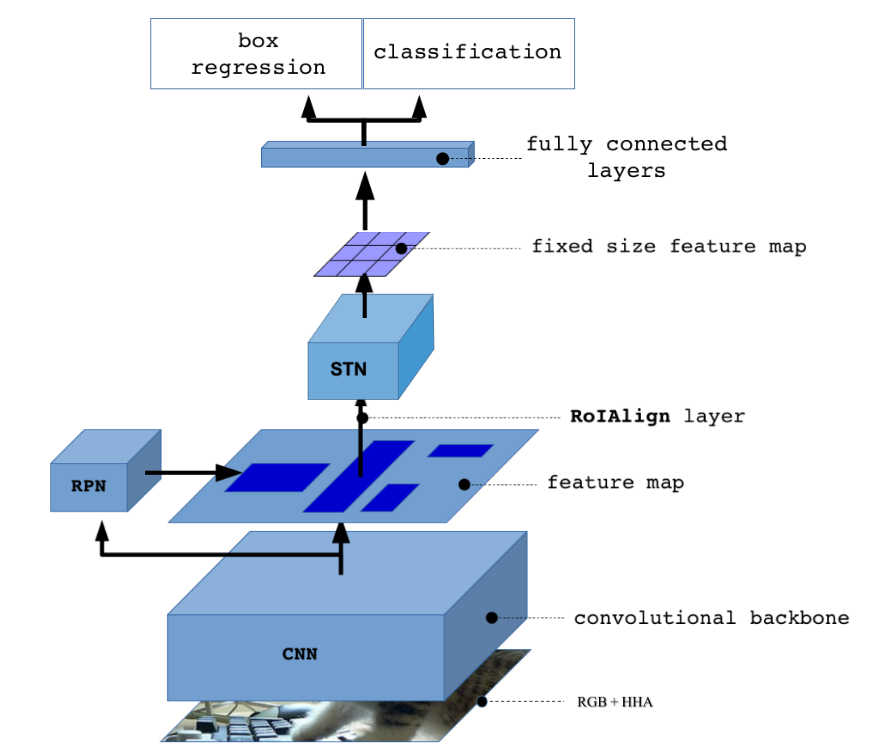
\includegraphics[width=13cm]{3dfasterrcnn}
  \caption{3D Faster R-CNN结构}
  \label{fig:3d_faster_rcnn}
\end{figure}

相比于Faster R-CNN,本文所提出的3D Faster R-CNN主要增加对深度信息的处理和Spatial Transformer,分别用于解决Faster R-CNN在实际应用时所不能解决的问题:
\begin{itemize}
\item 难以检测出缺少纹理的物体
\item 对物体的旋转敏感,提取的特征不具有旋转不变性
\end{itemize}

对于缺少纹理的物体,单从RGB图中很难检测出目标,这是一个很显然的问题,但是现在我们可以从对偶RGB-D相机中获取深度图,对于纹理少的物体,可以从深度图中提取特征检测出目标,所以现在的关键问题是如何从深度图中提取特征,并结合到Faster R-CNN中,本文所提出的方法是将深度图转换到HHA,然后再使用CNN提取特征,具体后文会详细介绍。

Faster R-CNN对于物体旋转敏感的问题,归根到底是因为CNN所提取的特征不具有旋转不变性,实际出现这种问题的情况,如图\ref{fig:cat}所示,
\begin{figure}[!ht]
  \centering
  \subfloat[检测旋转前的图片]{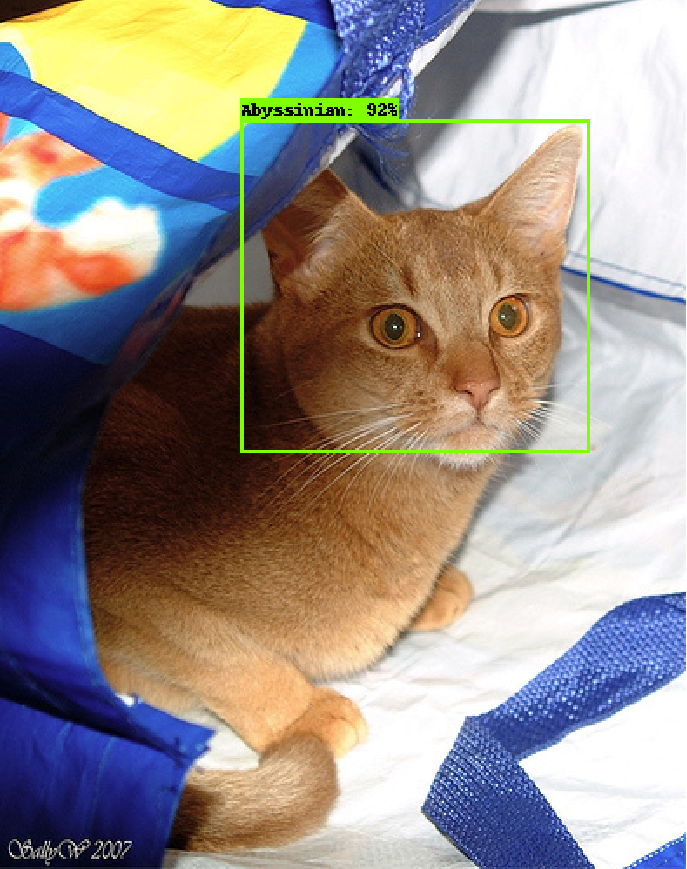
\includegraphics[width=4cm]{cat_up}}
  \hskip1em
  \subfloat[检测旋转后的图片]{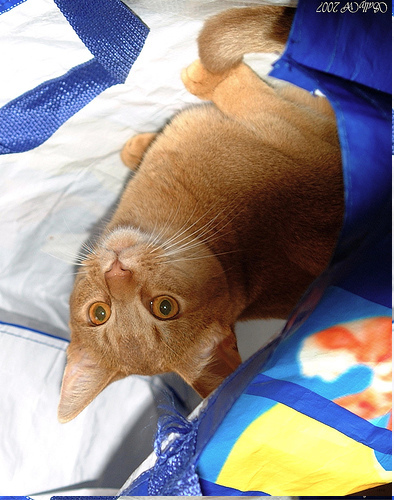
\includegraphics[width=4cm]{cat_down}}
  \caption{Faster R-CNN检测识别宠物猫示例}
  \label{fig:cat}
\end{figure}
其中图(b)只是将图(a)旋转了180度,由于CNN所提取的特征不具有旋转不变性,并且训练所实验的图片中的宠物都是头朝上的,即使图(a)在训练集中,将其旋转180度后,也无法从中检测出目标来。解决这个问题有两个思路:
\begin{itemize}
\item Data Augmentation
\item Spatial Transformer
\end{itemize}
Data Augmentation是通过对训练集中的图片进行旋转以获取不同角度的图片,通过这种方式增大数据集从而使得最终训练得到的模型对各种角度的图片都能识别;Spatial Transformer是一种特殊的网络结构,本文所使用的就这种方式,后文会详细介绍。

\subsection{Faster R-CNN}
为了更好地介绍所提出的3D Faster RCNN算法,先回顾一下Faster R-CNN算法。Faster R-CNN的网络结构如图\ref{fig:faster_rcnn}所示,
\begin{figure}[ht]
  \centering
  % @improve: more specific
  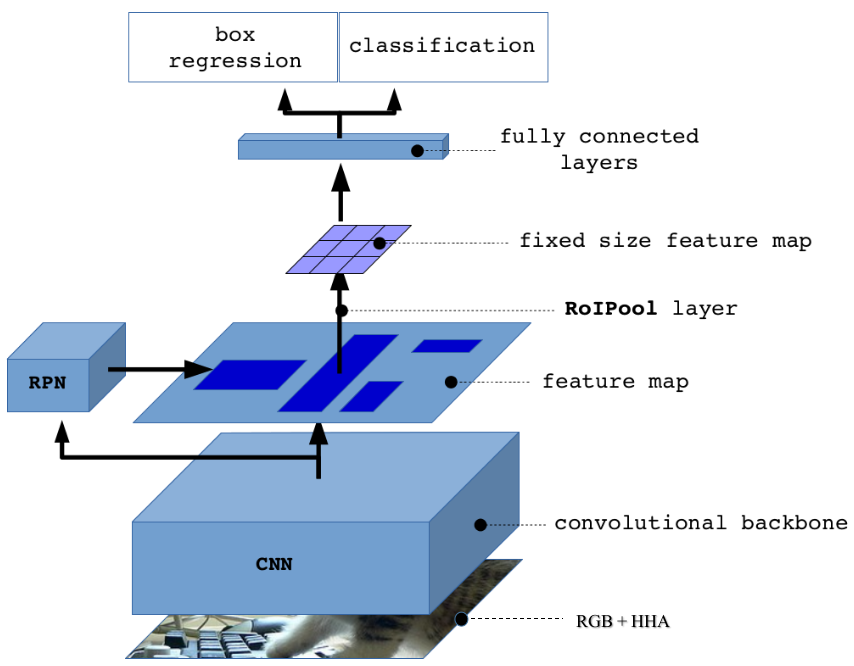
\includegraphics[width=13cm]{fasterrcnn}
  \caption{Faster R-CNN结构}
  \label{fig:faster_rcnn}
\end{figure}
Faster R-CNN的由两个核心模块构成:
\begin{itemize}
\item RPN(Region Proposal Network)
\item Fast R-CNN
\end{itemize}
整个网络是一个端到端(end-to-end)的目标检测网络,输入图片,输出图片中检测到的目标的类别和Bounding Box。RPN模块输出候选框,形象地说,RPN模块告诉Fast R-CNN模块去哪里检测目标,Fast R-CNN模块输出检测结果。

% @improve: faster r-cnn more specific ?


\subsection{HHA}
\label{sec:hha}
有了与彩色图对应的深度图,如何有效地利用深度图是一个值得思考的问题。从2012年AlexNet\cite{Krizhevsky2012}在ImageNet\cite{imagenet}数据集上的应用开始,深度学习在计算机视觉领域其准确率相比传统方法有了一个很大的提升,因此,本文考虑通过深度学习的方法结合深度图和彩色图进行目标检测。深度学习在彩色图上的应用已经相当成熟,但对于深度图的应用还比较少,如何使用CNN在深度图上提取特征也是一个值得探讨的问题,是将深度图直接作为一个通道使用CNN提取特征?还是将深度图变换到三维坐标(x,y,z),然后再在这三个通道上通过CNN提取特征?经过实验和相关调研,发现将深度图转换为HHA图后进行训练的模型有较高的准确率\cite{Gupta2014},因此本文将深度图转换为HHA三个通道,然后再通过CNN提取特征。HHA三个通道分别为:
\begin{itemize}
\item 水平方向上视差(Horizontal disparity)
\item 距离地面的高度(Height above ground)
\item 法向量与重力的夹角(Angle with gravity)
\end{itemize}
\textbf{Horizontal disparity:}深度图到视差的转换相对来说十分简单,理论上视差与深度呈倒数关系,因此水平方向上的视差计算具体如算法\ref{alg:hd}所示。
\begin{algorithm}[!ht]
  \caption{计算水平方向上视差}
  \label{alg:hd}
  \KwIn{Depth Frame $D_{h\times w}$}
  \KwOut{Horizontal disparity Frame $H_{h\times w}$}
  $h_{floor} = 1 / d_{ceil}, h_{ceil} = 1 / d_{floor}$\;
  \For {$y\leftarrow 1$ \KwTo $h$} {
    \For {$x\leftarrow 1$ \KwTo $w$} {
      $H[y, x] = 1 / D[y, x]$\;
      $H[y, x] = (H[y, x] - h_{floor}) / (h_{ceil} - h_{floor})$\;
    }
  }
\end{algorithm}

\textbf{Height above ground:}计算距离地面的高度首先要确定一个世界坐标系,然后得到世界坐标系到相机坐标系的旋转矩阵$\prescript{W}{C}{R}$和平移向量$\prescript{W}{C}{T}$,最后通过坐标变换得到距离地面的高度,具体如算法\ref{alg:hg}所示。
\begin{algorithm}[!ht]
  \caption{计算距离地面的高度}
  \label{alg:hg}
  \KwIn{Point Cloud $P_{h\times w}$}
  \KwOut{Hight Frame $H_{h\times w}$}
  \For {$y\leftarrow 1$ \KwTo $h$} {
    \For {$x\leftarrow 1$ \KwTo $w$} {
      $p =  \prescript{W}{C}{R}P[y, x] + \prescript{W}{C}{T}$\;
      $H[y, x] = p.z$\;
    }
  }
\end{algorithm}

\textbf{Angle with gravity:}法向量与重力的夹角的计算相对来说稍微复杂一点,重力的方向在工作区间内一般与所设的世界坐标系的$z$轴负方向相同,因此原问题就是求法向量与世界坐标系$z$轴负方向之间的夹角。参考文献\cite{Gupta2013},首先计算深度图中每个点上的法向量,计算点云中一点$p_0$的法向量$\vec{n}$的简单思路如下:
\begin{itemize}
\item 找出距离点$p_0$最近的$k$个点:$p_1, p_2,...p_k$
\item 通过最小二乘在点$\{p_i|i = 0, 1, \ldots , k\}$中拟合出平面$Ax + By + Cz + D = 0$
\item 点$p_0$的法向量$\vec{n} = [A, B, C]^T$
\end{itemize}
考虑到所采集的深度图转换的点云是有序的(Organized Point Cloud),意味着坐标索引相近的点实际物理距离也相近,因此找出距离点$p_0$最近的$k$个点可以通过选取点$p_0$坐标索引附近的点代替,具体地,记点$p_0$在深度图中图像坐标为$(x_0, y_0)$,取点集$\bm{S} = \{p_i|x_0 - R \leq x_i \leq x_0 + R , y_0 -R \leq y_i \leq y_0 + R\}$,其中$R$是选取区域的半径。得到法向量后计算法向量与世界坐标$z$轴负方向的角度就十分简单了,整个计算法向量与重力的夹角的算法如\ref{alg:angle}所示。
\begin{algorithm}[!ht]
  \caption{计算法向量与重力的夹角}
  \label{alg:angle}
  \KwIn{Point Cloud $P_{h\times w}$}
  \KwOut{Angle Frame $A_{h\times w}$}
  \For {$y\leftarrow 1$ \KwTo $h$} {
    \For {$x\leftarrow 1$ \KwTo $w$} {
      Calculate surface normal $\prescript{C}{}{\vec{n}}$ at point $P[y,x]$\;
      $\prescript{W}{}{\vec{n}} =  \prescript{W}{C}{R}\prescript{C}{}{\vec{n}} + \prescript{W}{C}{T}$\;
      $A[y, x] = arccos(-(\vec{n}\cdot\vec{oz}) / (|\vec{n}||\vec{oz}|))$\;
    }
  }
\end{algorithm}

计算完上述HHA三个通道后,为了计算和存储方便,分别将三个通道的值线性变换到0到255之间,可视化如图\ref{fig:hha}所示。
\begin{figure}
  \centering
  \subfloat[Depth frame]{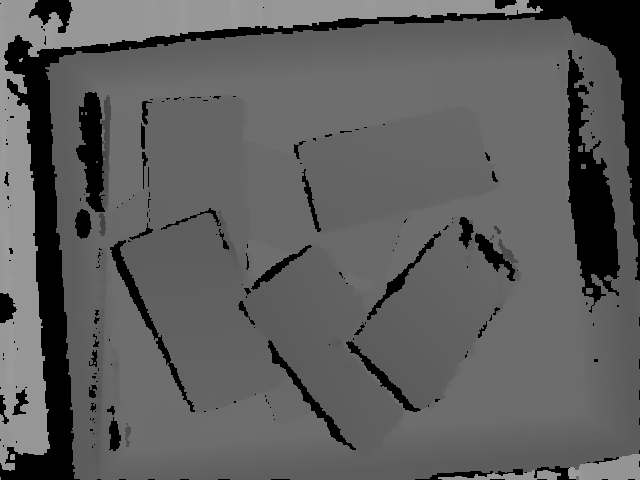
\includegraphics[width=4.5cm]{depth_frame}}
  \hskip5em
  \subfloat[HHA frame]{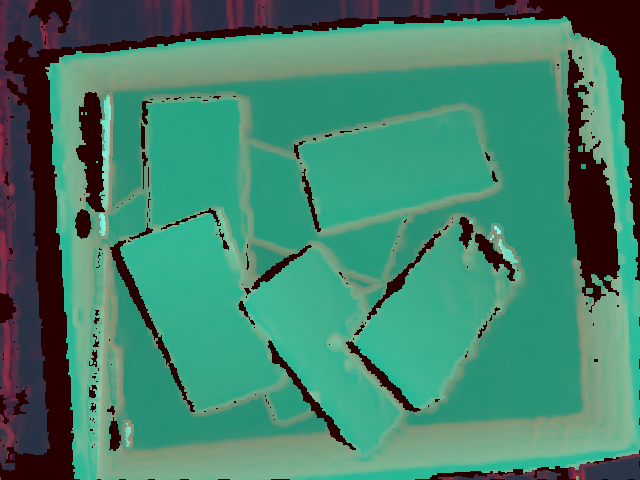
\includegraphics[width=4.5cm]{hha_frame}}
  \vfill
  \subfloat[Horizontal disparity frame]{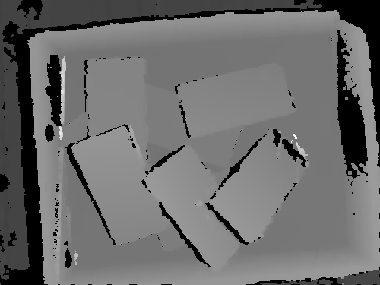
\includegraphics[width=4.5cm]{disparity_frame}}
  \hfill
  \subfloat[Height above ground frame]{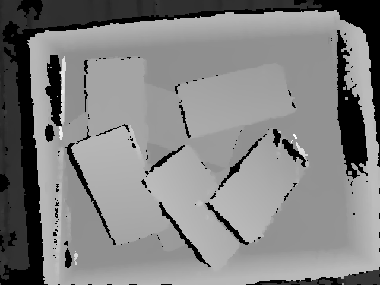
\includegraphics[width=4.5cm]{height_frame}}
  \hfill
  \subfloat[Angle with gravity frame]{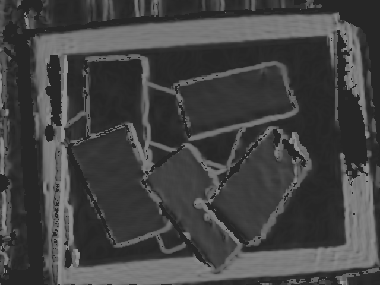
\includegraphics[width=4.5cm]{angle_frame}}
  \caption{HHA可视化效果图}
  \label{fig:hha}
\end{figure}

\subsection{Spatial Transformer}
Spatial Transformer是一个可微模块,根据输入的特征对其进行相应的空间变化,输出变换后的特征,如图\ref{fig:spatial_transformer_results}所示,
\begin{figure}[ht]
  \centering
  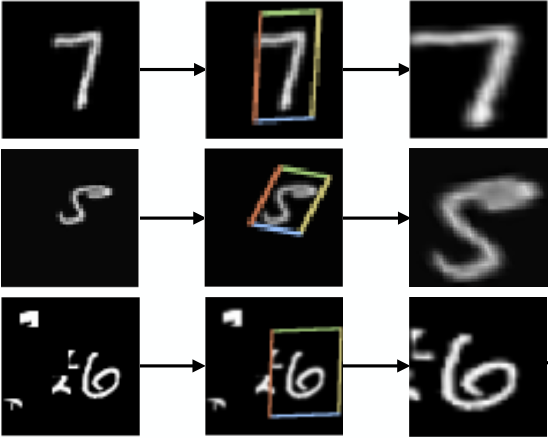
\includegraphics[width=6cm]{stn_results}
  \caption{Spatial Transformer效果图}
  \label{fig:spatial_transformer_results}
\end{figure}
输入特征$U$经过Spatial Transformer模块后输出特征$V$。Spatial Transformer模块具体可以分为三个部分,如图\ref{fig:spatial_transformer}。
\begin{figure}[ht]
  \centering
  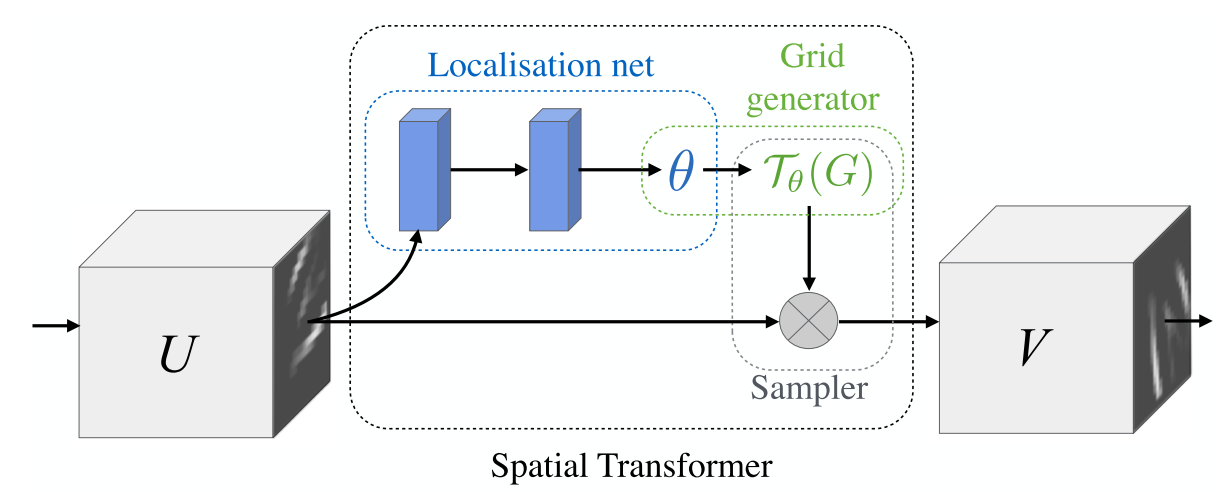
\includegraphics[width=12cm]{stn_structure}
  \caption{Spatial Transformer结构图}
  \label{fig:spatial_transformer}
\end{figure}
简单来讲,第一部分是一个定位网络(localisation network),输入特征$U$,输出需要进行空间变换的参数;第二部分是一个网格生成器(grid generator),根据空间变换的参数生成输入特征中需要变换的点的网格;第三部分是个采样器,根据网格生成器的输出对输入特征进行采样并进行空间变换,生成输出特征。

具体地,记定位网络的输入为特征$U\in \mathbb{R}^{H\times W\times C}$,其中$W,H,C$分别为长、宽和通道数,网络的输出为空间变化$\mathcal{T}_{\theta}$的参数$\theta$,参数$\theta$的个数由空间变换的类型决定,本文所采用的空间变换为2D仿射变换,则
\begin{equation}
  \mathcal{T}_\theta = \left[
    \begin{array}{ccc}
      \theta_{11}&\theta_{12}&\theta_{13}\\
      \theta_{21}&\theta_{22}&\theta_{23}
    \end{array}
    \right]
\end{equation}
定位网络内部可以由一些全连接层或者卷积层再加一个回归层组成。

网格生成器本质上就是在输入特征中选取需要进行空间变化的点,如图\ref{fig:spatial_transfomer_results}中绿色点便是网格生成器所选取的点,记Spatial Transformer的输出特征为$V\in \mathbb{R}^{H'\times W'\times C}$,其中$W',H',C$分别为输出特征的长、宽和通道数,输出特征的通道数和输入特征的通道数相同,不能改变,并且空间变换$\mathcal{T}_{\theta}$将分别作用于输入$U$的各个通道以保证每个通道上的变换一致。并记点集$G = \{G_i|G_i = (x^t_i, y^t_i)\}$,其中$(x_i^s, y_i^s)$为输出特征图中点的坐标,由定位网络输出的参数$\theta$和$G$我们就可以在输入特征中确定需要进行空间变换的点的集合$\mathcal{T}_\theta(G)$:
\begin{equation}
  \left(
    \begin{array}{c}
      x_i^s\\
      y_i^s
    \end{array}
  \right) = \mathcal{T}_\theta(G_i) =
  \left[
    \begin{array}{ccc}
    \theta_{11}&\theta_{12}&\theta_{13}\\
    \theta_{21}&\theta_{22}&\theta_{23}
    \end{array}
  \right]
  \left(
    \begin{array}{c}
      x_i^t\\
      y_i^t\\
      1\\
    \end{array}
  \right)
\end{equation}
其中$(x_i^s, y_i^s)$是输入特征中点的坐标,也是图\ref{fig:spatial_transfomer_result}中的绿色点。

采样器输入网格生成器生成的点集$\mathcal{T}_\theta$,和输入特征$U$,最终输出经过空间变换后的特征$V$,具体如公式\ref{eq:sampler}所示:
\begin{equation}
  \label{eq:sampler}
  V_i^c = \sum_n^H\sum_m^W{U_{nm}^ck(x_i^s-m;\Phi_x)k(y_i^s-n;\Phi_y)}\quad \forall i\in[1\ldots H'W']\quad \forall c\in[1\ldots C]
\end{equation}
其中$\Phi_{x}$和$\Phi_{y}$是采样核函数$k()$的参数,$U_{nm}^c$表示输入特征$U$在坐标$(n, m)$下第$c$个通道上的值,$V_i^c$表示输出特征在坐标$(x_i^t,y_i^t)$下第$c$个通道上的值。理论上可以使用任何采样核函数,只要可以对$x_i^s$和$y_i^s$求导,因为网络训练需要对公式\ref{eq:sampler}求导。以双线性采样核函数为例,公式\ref{eq:sampler}变为
\begin{equation}
  V_i^c = \sum_n^H\sum_m^W{U_{nm}^cmax(0, 1-|x_i^s-m|)max(0, 1-|y_i^s-n|)}
\end{equation}
则$V$对$U$和$G$的梯度为
\begin{equation}
  \frac{\partial V_i^c}{\partial U_{nm}^c} = \sum_n^H\sum_m^W{max(0, 1-|x_i^s-m|)max(0, 1-|y_i^s-n|)}
\end{equation}
\begin{equation}
  \frac{\partial V_i^c}{\partial x_i^s} = \sum_n^H\sum_m^W{U_{nm}^cmax(0, 1-|y_i^s-n|)}
  \left\{
      \begin{array}{ll}
        0&if\; |m-x_i^s| \geq 1\\
        1&if\; m \geq x_i^s\\
        -1&if\; m < x_i^s
      \end{array}
    \right.
\end{equation}
\begin{equation}
  \frac{\partial V_i^c}{\partial y_i^s} = \sum_n^H\sum_m^W{U_{nm}^cmax(0, 1-|x_i^s-m|)}
  \left\{
      \begin{array}{ll}
        0&if\; |n-y_i^s| \geq 1\\
        1&if\; n \geq y_i^s\\
        -1&if\; n < y_i^s
      \end{array}
    \right.
\end{equation}


\section{3D Mask R-CNN}
Mask R-CNN相比Faster R-CNN不仅可以输出目标的Class和Bounding Box,还可以输出目标的Mask。Mask R-CNN相比Faster R-CNN主要的技术要点有:
\begin{itemize}
\item 强化了特征提取网络
\item 采用ROIAlign代替ROIPooling
\item Mask的损失函数
\end{itemize}
因此3D Mask R-CNN也针对上述三个要点对3D Faster R-CNN进行改进,其结构框架如图\ref{fig:3d_mask_rcnn}所示。
\begin{figure}[ht]
  \centering
  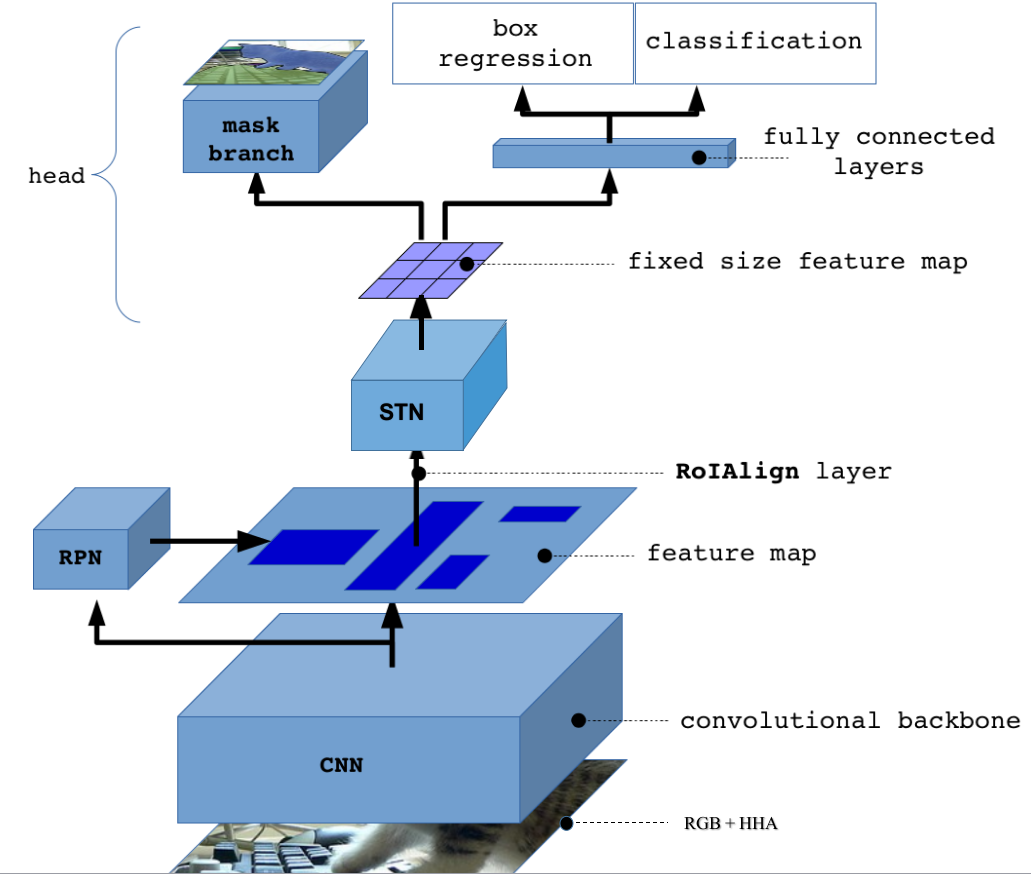
\includegraphics[width=13cm]{3dmaskrcnn}
  \caption{3D mask R-CNN结构}
  \label{fig:3d_mask_rcnn}
\end{figure}

\subsection{特征提取网络}
3D Faster R-CNN的特征提取网络使用的是VGG-16\cite{simonyan2014very},VGG16是牛津大学VGG组提出的。VGG16相比最早的AlexNet的一个改进是采用连续的几个$3\times 3$的卷积核代替AlexNet中的较大卷积核($11\times 11$,$5\times 5$)。对于给定的感受野(与输出有关的输入图片的局部大小),采用堆积的小卷积核是优于采用大的卷积核,因为多层非线性层可以增加网络深度来保证学习更复杂的模式,而且代价还比较小(参数更少)。比如,3个步长为1的$3\times 3$卷积核连续作用在一个大小为7的感受野,其参数总量为$3\times 9C^2$,其中$C$是通道数,如果直接使用$7\times 7$卷积核,其参数总量为$49C^2$。而且$3\times 3$卷积核有利于更好地保持图像性质。

3D Mask R-CNN改用了ResNeXt-101+FPN网络提取特征,该网络主要由ResNeXt\cite{xie2017aggregated}和FPN\cite{lin2017feature}两部分构成。ResNeXt是对残查网络ResNet\cite{he2016deep}的改进,在介绍ResNeXt之前先介绍一下ResNet。ResNet为了解决随着网络层数增加,靠前的层梯度会很小,导致训练时学习停滞、梯度消失的问题,引入了残差模块,如图\ref{fig:resnet}所示。
\begin{figure}[ht]
  \centering
  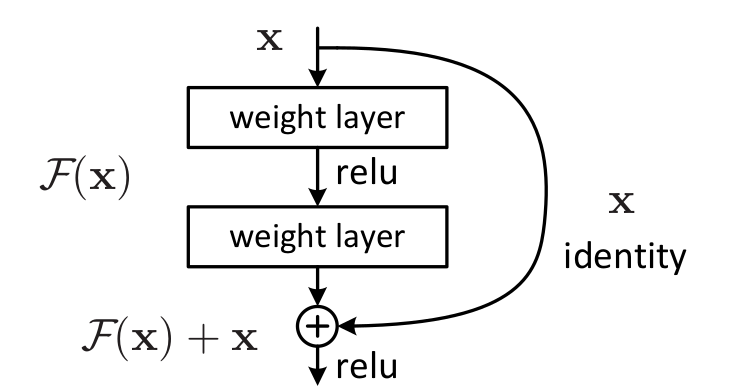
\includegraphics[width=8cm]{resnet}
  \caption{残差模块}
  \label{fig:resnet}
\end{figure}
残差单元可以解决学习停滞问题的背后逻辑在于此:想象一个网络A,其训练误差为$x$。现在通过在A上面堆积更多的层来构建网络B,这些新增的层什么也不做,仅仅复制前面A的输出。这些新增的层称为C。这意味着网络B应该和A的训练误差一样。那么,如果训练网络B其训练误差应该不会差于A。但是实际上却是更差,唯一的原因是让增加的层C学习恒等映射并不容易。为了解决这个退化问题,残差模块在输入和输出之间建立了一个直接连接,这样新增的层C仅仅需要在原来的输入层基础上学习新的特征,即学习残差,会比较容易。ResNeXt在ResNet的基础上,提出cardinality的概念,如图\ref{fig:resnext},
\begin{figure}[ht]
  \centering
  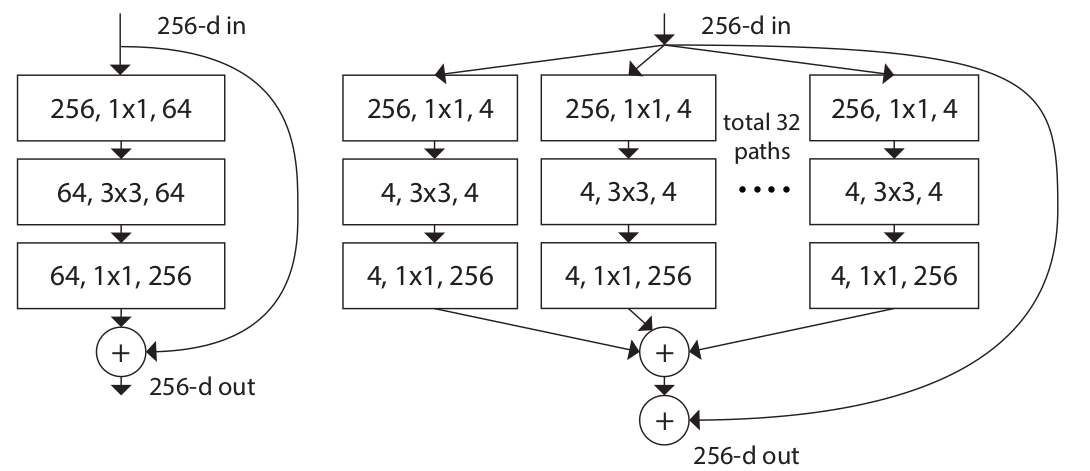
\includegraphics[width=10cm]{resnext}
  \caption{ResNeXt对ResNet的改进}
  \label{fig:resnext}
\end{figure}
其中左右两个网络结构有相同的参数个数,左边是ResNet的一个区块,右边的ResNeXt中每个分支一模一样,分支的个数就是cardinality,其通过在大卷积核层两侧加入$1\times 1$的网络层来控制核个数、减少参数个数。因此,与ResNet相比,相同的参数个数,ResNeXt结果更好:一个101层的ResNeXt网络,和200层的ResNet准确度差不多,但是计算量只有后者的一半。

\subsection{ROIAlign}
ROIPooling采用的是最近领插值(Nearest neighbor interpolation),即在resize时,对于缩放后坐标不能刚好为整数的情况,采用四舍五入的方法,相当于选取离目标点最近的点。虽然这种处理方法对分类问题影响不大,但是现在Mask R-CNN需要预测Pixel级别的Mask,ROIPooling造成的像素不对齐问题对Mask的精确度影响很大,因此提出ROIAlign代替ROIPooling,ROIAlign使用双线性插值(Bilinear interpolation)来获得像素级别的对齐。举例来说,假设在$8\times 8$的特征图中提取提取$2\times 2$的输出,ROIPooling的示意图如\ref{fig:roipooling}所示,ROIAlign的示意图如\ref{fig:roialign}所示。

\begin{figure}[ht]
  \centering
  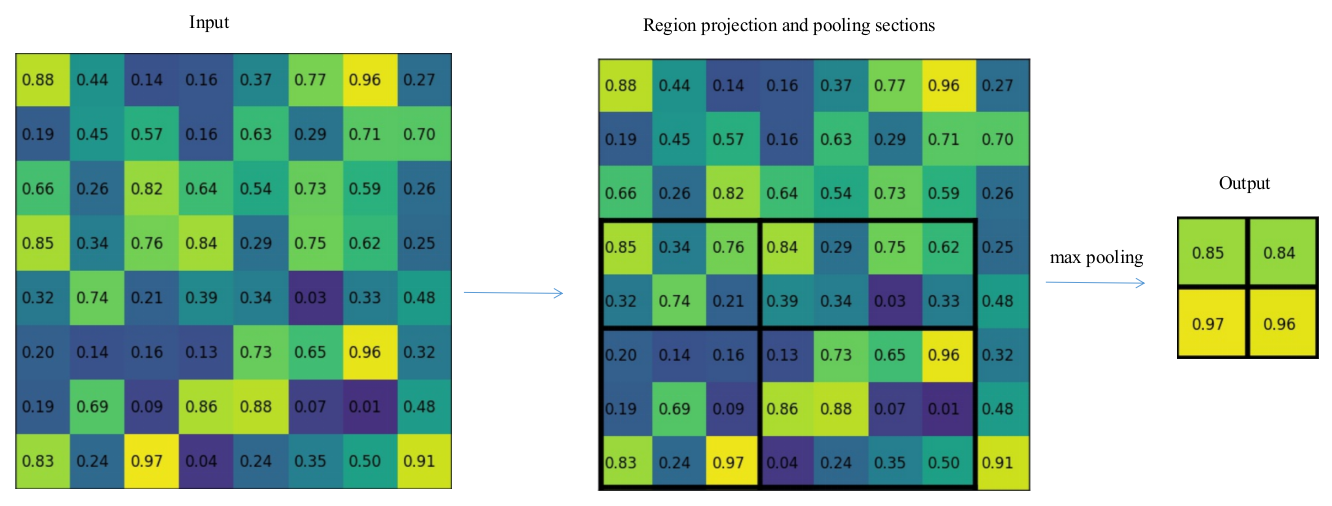
\includegraphics[width=13cm]{roipooling}
  \caption{ROIPooling示意图}
  \label{fig:roipooling}
\end{figure}
\begin{figure}[ht]
  \centering
  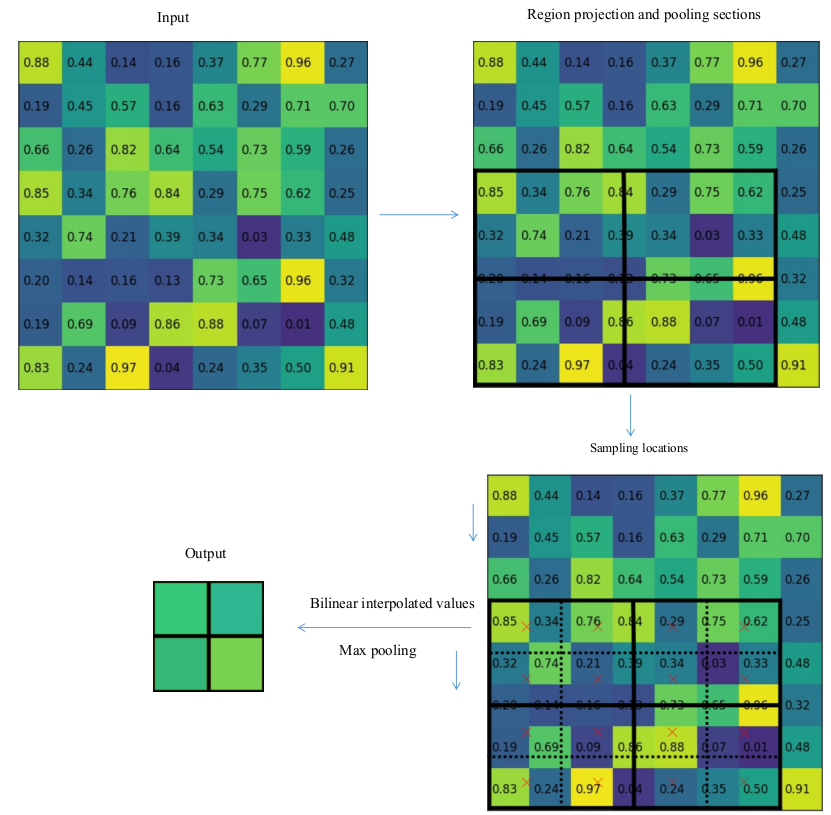
\includegraphics[width=10cm]{roialign}
  \caption{ROIAlign示意图}
  \label{fig:roialign}
\end{figure}

\subsection{Mask损失函数}
为了有效的避免类之间的竞争,使得其他class不贡献损失,Mask的损失函数使用平均二值交叉熵(average binary cross-entropy)。具体的,对于每个ROIAlign的$K\times m^2$维输出,$K$表示总类别个数,$m$对应mask分辨率,即输出$K$个mask,定义Mask的损失函数为
\begin{equation}
  L_{mask} = -\frac{1}{K}\sum_{i=1}^K{\sum_j{(y_j'\lg(y_j)+(1-y_j')\lg(1-y_j))}}
\end{equation}
其中
\begin{equation}
  j = 1,2,\ldots,m^2
\end{equation}
表示mask的像素索引。通过上述损失函数的定义有效的避免了类间的竞争,将mask分支与class分支并行区分开来,通过class分支最终的输出在$K$个mask中选择对应的mask输出。实验表明,相比将mask和class混在一起,根据mask的结果来判断类别的方法,这种方法对算法最终的精确度有着重要意义。

\section{目标检测实验}
为了评价所设计的3D Faster R-CNN和3d Mask R-CNN算法的性能,分别在一个现有的数据集和一个自己采集的实际应用的数据集上进行了网络的训练和测试,并与原始的Faster R-CNN和Mask R-CNN相比较,验证了所设计算法的性能。

\subsection{数据集}
\label{sec:dataset}
实验所采用的数据集一个是参加APC(Amazon Picking Challenge)的MIT-Princeton队伍所采集的数据集"Shelf \& Tote" Benchmark Dataset\cite{apcdataset},此处简单记为APC数据集,另外一个数据集是实际用于bin-picking在实验室采集的数据集,记为workpiece数据集。

{\kai APC数据集:}该数据集共有39类不同的物体,452个场景,每个场景有不同的物体,一共7281组图片,通过在多个场景下,不同的视角下使用Intel Realsense SR300相机所拍摄。标注的数据是每个场景下物体在世界坐标系下的位姿,以及每个场景下相机在世界坐标系下的位姿,是一个半自动标注的数据集,通过物体的位姿和相机的位姿就可以得到每个物体在相机坐标系下的位姿,数据集中部分数据如图\ref{fig:apc_dataset}所示。
\begin{figure}[ht]
  \centering
  \subfloat{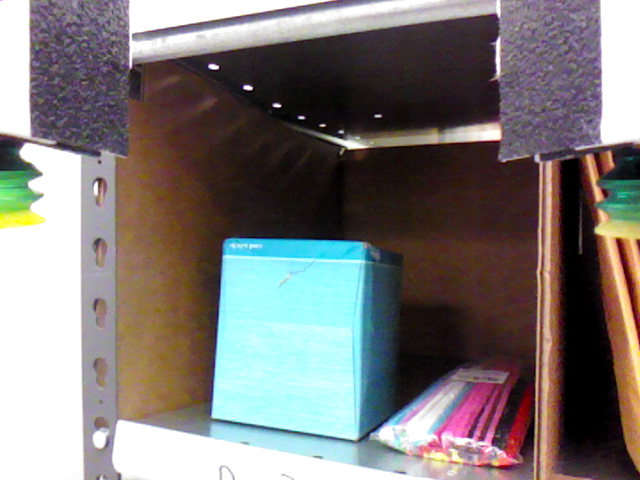
\includegraphics[width=3.5cm]{apc_color1}}
  \hskip0.2cm
  \subfloat{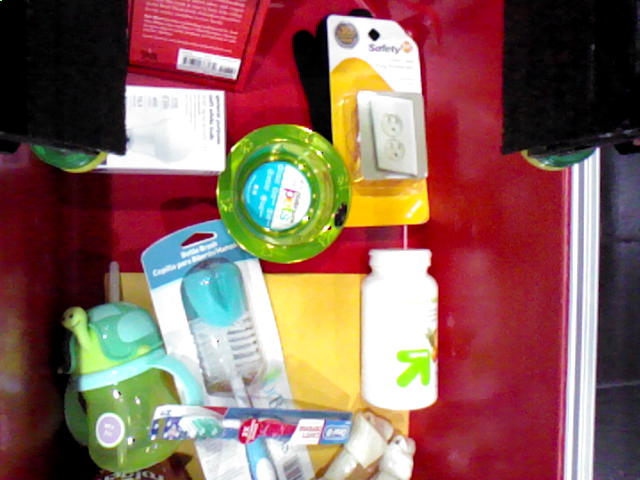
\includegraphics[width=3.5cm]{apc_color2}}
  \hskip0.2cm
  \subfloat{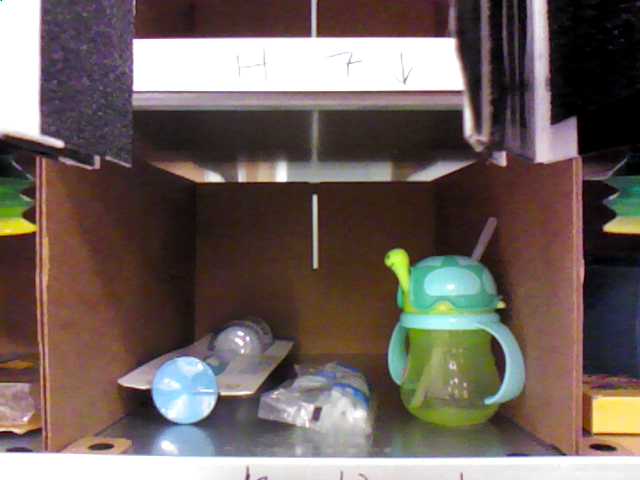
\includegraphics[width=3.5cm]{apc_color3}}
  \hskip0.2cm
  \subfloat{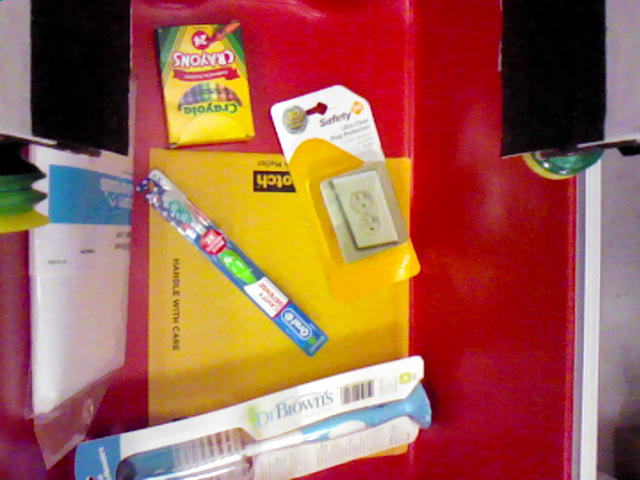
\includegraphics[width=3.5cm]{apc_color4}}
  \vfill
  \subfloat{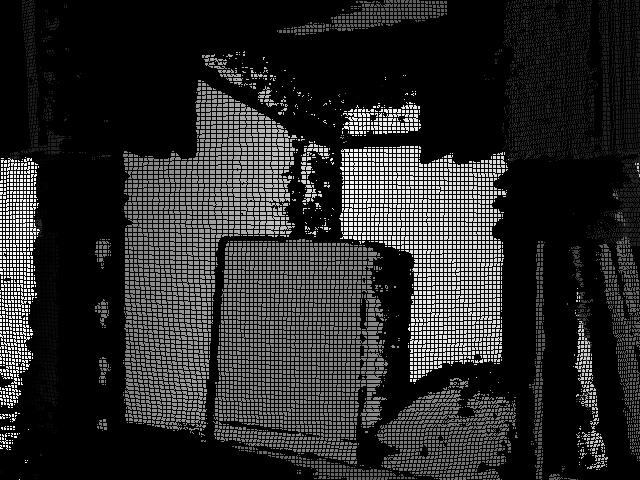
\includegraphics[width=3.5cm]{apc_depth1}}
  \hskip0.2cm
  \subfloat{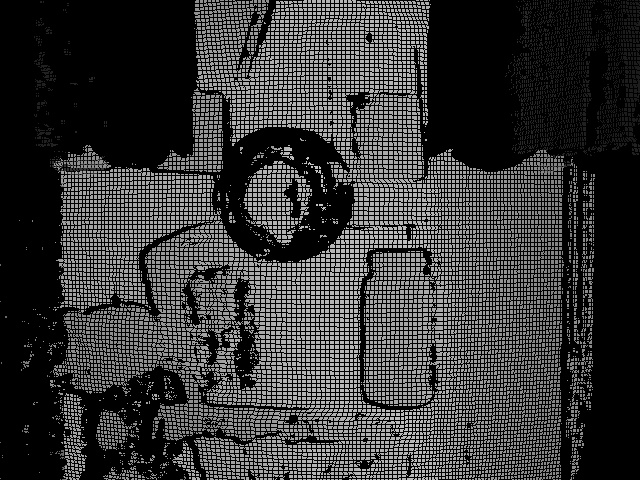
\includegraphics[width=3.5cm]{apc_depth2}}
  \hskip0.2cm
  \subfloat{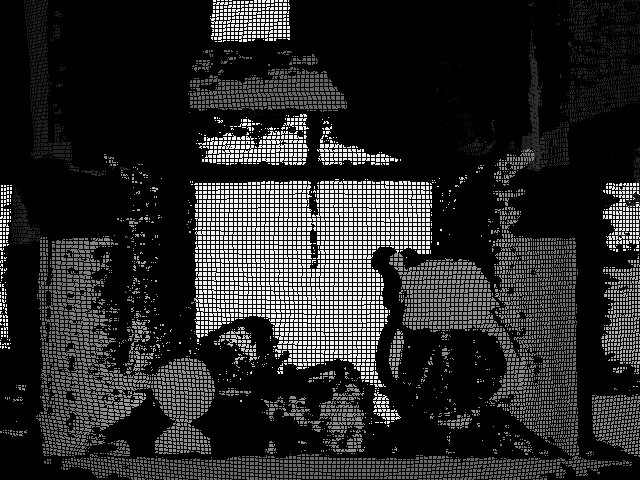
\includegraphics[width=3.5cm]{apc_depth3}}
  \hskip0.2cm
  \subfloat{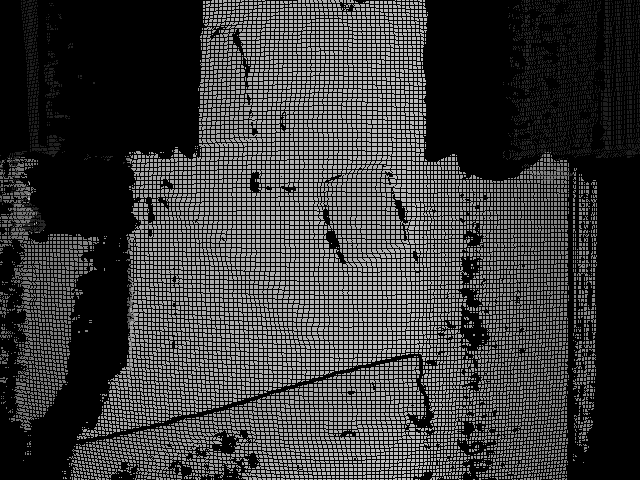
\includegraphics[width=3.5cm]{apc_depth4}}
  \caption{APC数据集部分数据:第一栏为彩色图像,第二栏为与彩色图像相匹配的深度图}
  \label{fig:apc_dataset}
\end{figure}

APC数据集中标注的标签可以认为是每个物体在相机坐标系下的位姿和类别,对于设计的算法来说需要的是物体的类别(class)、边界框(bounding box)和掩模(mask),因此需要对原始标注数据进行一些处理,因为APC还提供了每类物体的CAD模型,并且相机的内参矩阵也在数据集中提供了,因此可以将CAD模型转换为点云后齐次变换到所标注的对应物体在相机坐标系下的位姿,然后利用相机内参矩阵将物体点云投影到图像平面,从而获得物体的mask,进而可以得到物体的bounding box。需要注意的是由于一个场景中有多个物体,在不同相机位姿下会出现遮挡,因此需要对被遮挡物体的mask进行相应的裁剪,对于几乎被完全遮挡的物体可以去除,判断物体是否遮挡可以通过物体点云距离相机原点的距离远近判断。将一张图中物体位姿得到mask和boudning box的处理流程如下所示:
\begin{enumerate}
\item 对于图中标注的每个物体:
  \begin{itemize}
  \item 将对应物体的3D点云变换到物体标注的位姿
  \item 根据相机内参矩阵将3D点云投影到图像平面,获得物体的mask以及mask对应的深度图depth
  \end{itemize}
\item 遍历像素索引i:
  \begin{itemize}
  \item 如果在索引i出存在多张mask的值有效,保留depth值最小的mask,将其余mask在索引i处置为无效
  \end{itemize}
\item 对于每个物体的mask:
  \begin{itemize}
  \item 如果mask中有效像素点小于阈值$T$,删除该mask
  \item 根据mask有效像素点的坐标计算对应的bounding box
  \end{itemize}
\end{enumerate}
处理后的部分图片的ground truth(class,mask,boudning box)如图\ref{fig:apc_gt}所示。
\begin{figure}[ht]
  \centering
  \subfloat{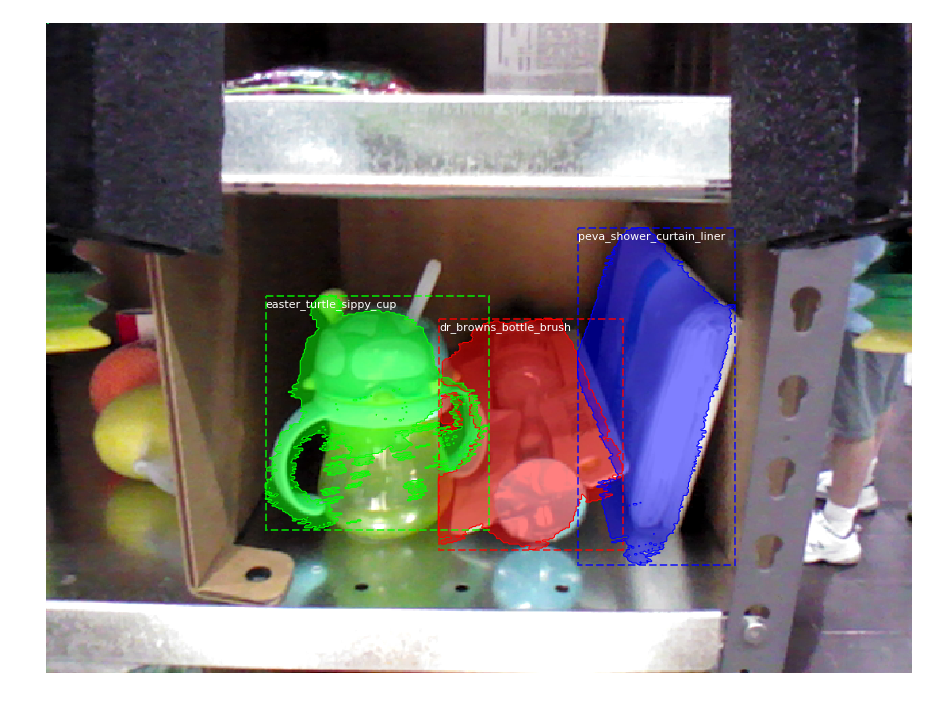
\includegraphics[width=6cm]{apc_gt1}}
  \hskip1cm
  \subfloat{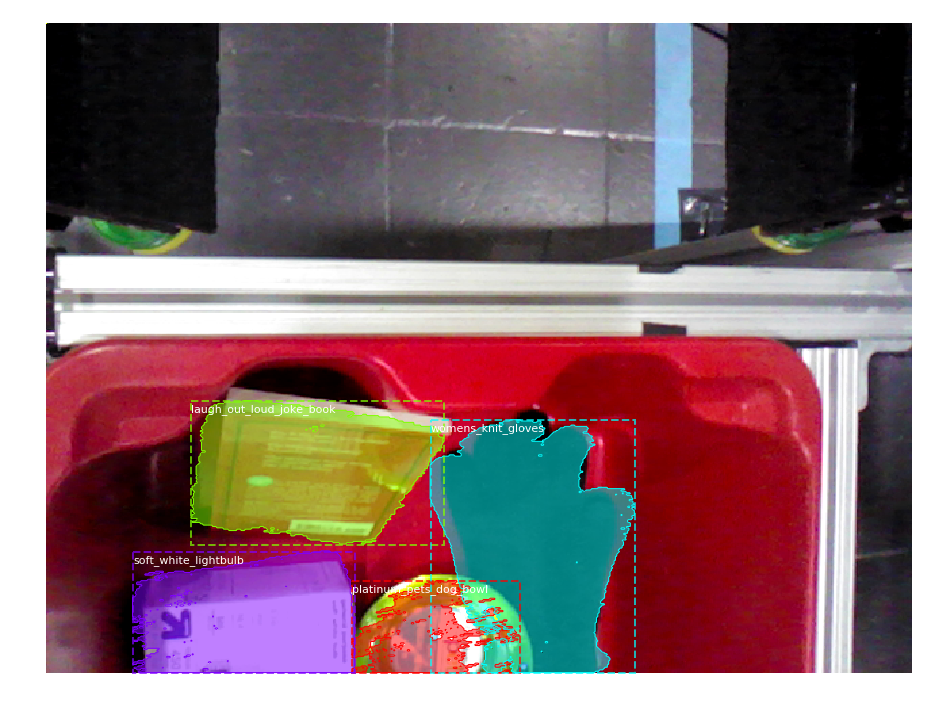
\includegraphics[width=6cm]{apc_gt2}}
  \vfill
  \subfloat{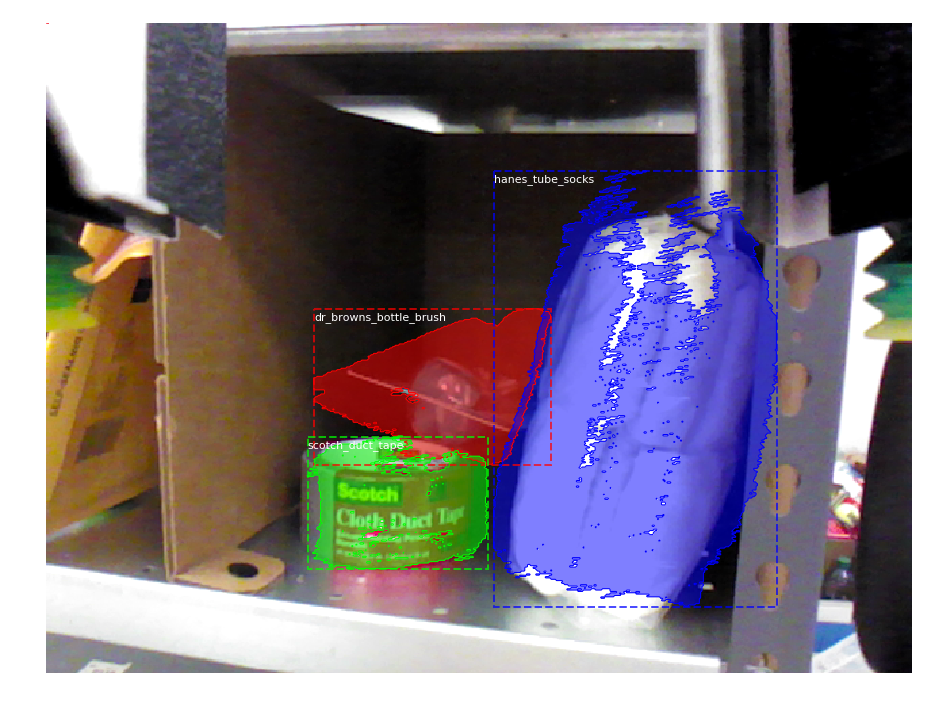
\includegraphics[width=6cm]{apc_gt3}}
  \hskip1cm
  \subfloat{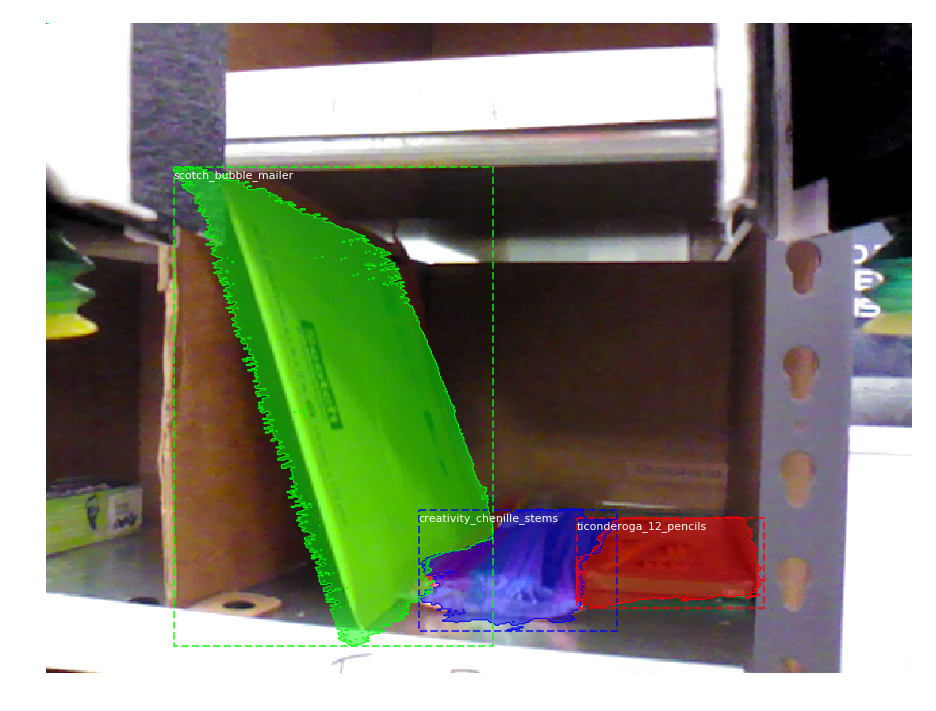
\includegraphics[width=6cm]{apc_gt4}}
  \caption{APC数据集部分标注数据}
  \label{fig:apc_gt}
\end{figure}
从图\ref{fig:apc_gt}可以看出处理后的mask基本覆盖了物体,boudning box也正确框出了物体,唯一的缺点是所生成的mask有时候有些缺失,没有人工标注的完美,如图\ref{fig:apc_gt}中第一张图中的瓶子(easter turtle sippy cup)标注的mask有很多缺失,根本原因是所使用的物体的CAD模型是通过相机采集生成的,其转换的3D点云质量并不是十分理想,其3D点云比较稀疏并且有部分缺失,如图\ref{fig:apc_model}所示,这个瓶子的点云有严重的缺失,主要原因是瓶子透明,所以相机难以采集其深度信息。
\begin{figure}[ht]
  \centering
  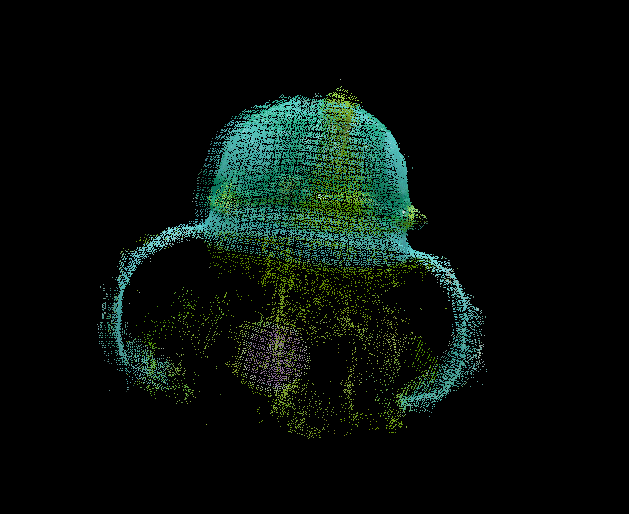
\includegraphics[width=10cm]{apc_model1}
  \caption{easter turtle sippy cup point cloud}
  \label{fig:apc_model}
\end{figure}
模型点云的缺失,因此将点云投影到图像平面生成的mask也有部分缺失,尽管已经对生成的mask进行了一些滤波处理,但部分mask还是有明显的缺失。

总体来说,尽管生成的ground truth的质量没有人工标注的ground truth质量好,但对本实验来说已经够用,并且相比人工标注这种半自动化的标注方式节省了大量时间和金钱成本。

{\kai workpiece数据集:} 该数据集有三类物体,共2k组图片。该数据集与APC数据集最大的不同是,同一张图片中存在大量不同位姿的同种物体,并且三类物体都缺少纹理(textureless),因此Faster R-CNN和Mask R-CNN在该数据集上的表现理论上应该大大不如3D Faster R-CNN和3D Mask R-CNN。部分数据集中的图片如图\ref{fig:wp_dataset}所示。
\begin{figure}[ht]
  \centering
  @todo: missing workpiece dateset figures
  \subfloat{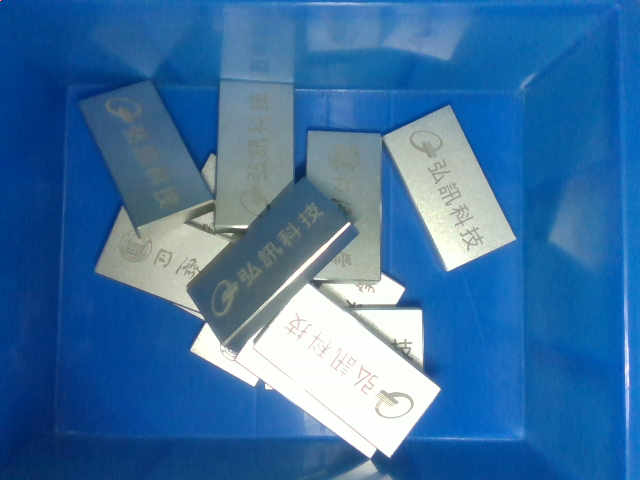
\includegraphics[width=3.5cm]{wp_color1}}
  \hskip0.2cm
  \subfloat{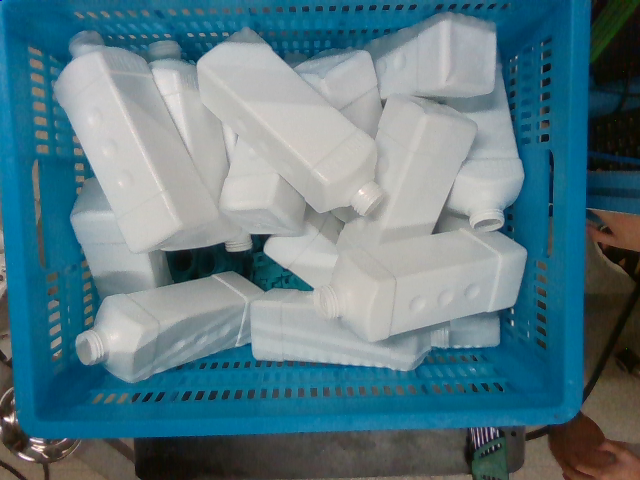
\includegraphics[width=3.5cm]{wp_color2}}
  \vfill
  \subfloat{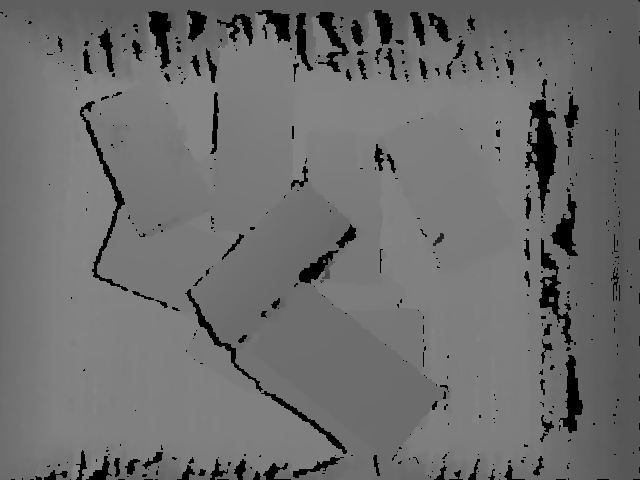
\includegraphics[width=3.5cm]{wp_depth1}}
  \hskip0.2cm
  \subfloat{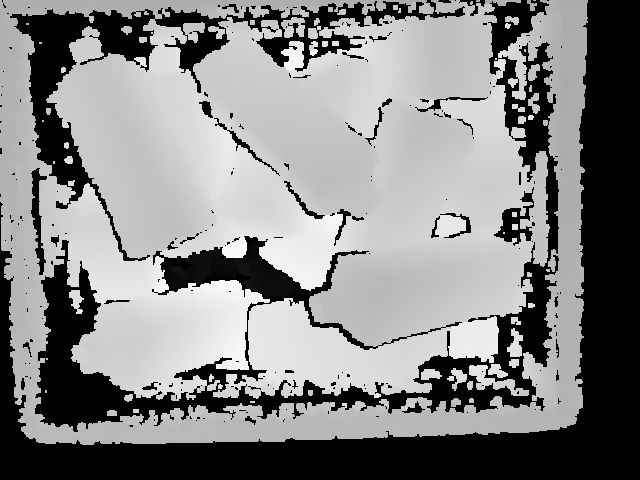
\includegraphics[width=3.5cm]{wp_depth2}}
  \caption{workpiece数据集部分图片}
  \label{fig:wp_dataset}
\end{figure}
workpiece数据集的ground truth由人工标定,其中据测试集中有的ground truth不仅包括了物体的class,mask,bounding box,还有物体的位姿,并且由于三类物体都是工厂中的工件,因此也提供三类物体精确的CAD模型。

\subsection{实验内容}
实验在APC数据集和workpiece数据集上比较Faster R-CNN和3D Faster R-CNN、Mask R-CNN和3D Mask R-CNN的性能。

{\kai 算法实现}主要通过Tensorflow框架使用python语言实现,详细代码见Github项目地址\footnote{\url{https://github.com/freealong/Mask\_RCNN}}。

{\kai 评价的指标}主要是检测的精确度AP以及算法的时间性能FPS。FPS是每秒能检测的图片数比较好理解,AP是bounding box或者mask交并比的精确度。具体地,如图\ref{fig:iou}所示,
\begin{figure}[ht]
  \centering
  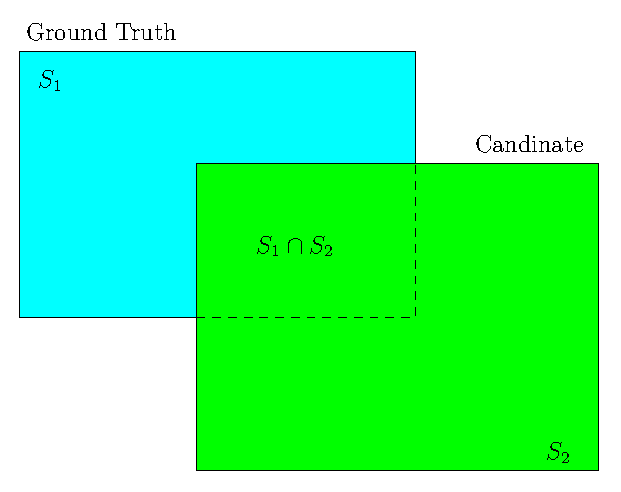
\includegraphics[width=8cm]{iou}
  \caption{bounding box交并比}
  \label{fig:iou}
\end{figure}
两个bounding box的交并比定义为:
\begin{equation}
  IoU = \frac{S_1\cap S_2}{S_1\cup S_2}
\end{equation}
$AP_{0.5}$表示检测的结果与ground truth的交并比大于0.5的个数占总体检测个数的比例,显然定义精度的$IoU$大小会影响最终评价的质量,过小和过大的最小$IoU$都不能很好地反应算法的精缺度,因此将评价的主要精确度定义如下:
\begin{equation}
  AP = \frac{1}{10}\sum_{i=0}^{9}{AP_{0.5 + 0.5i}}
\end{equation}
检测结果换为mask精确度的定义也类似,只需用mask的交并比代替bounding box的交并比。

{\kai 模型训练}在实验室的服务器上进行,服务器有两块Intel(R) Xeon(R) E5-2683 v3(2.00GHz)的CPU,4块TITAN X GPU。模型训练时为了减少训练时间,4块GPU都使用了。在APC数据集上,训练用了约6k组图片,剩下的1k多组图片用于测试,3D Faster R-CNN训练用了40个小时左右,3D Mask R-CNN用了48个小时左右;在workpiece数据集上,训练用了约1.6k组图片,剩下的400组图片用于测试,3D Faster R-CNN训练用了30个小时左右,3D Mask R-CNN用了36小时左右。

\subsection{实验结果}
在APC数据集上,本文算法Faster R-CNN和Mask R-CNN的精确度如表\ref{tab:ap1}所示,在测试集上的部分图片检测结果见图\ref{fig:ap_res}。
\begin{table}[ht]
  \centering
  \caption{算法在APC数据集上的精确度}
    \begin{tabular}{cccccc}
      \toprule
      &input&output&$AP$&$AP_{0.5}$&$AP_{0.75}$ \\
      \midrule
      Faster R-CNN&RGB&bbox&33.26&56.29&34.03 \\
      \bf{3D Faster R-CNN}&RGB+HHA&bbox&\bf{34.55}&\bf{57.99}&\bf{34.69} \\
      Mask R-CNN&RGB&mask&32.34&55.78&33.12 \\
      \bf{3D Mask R-CNN}&RGB+HHA&mask&\bf{33.94}&\bf{56.45}&\bf{33.99} \\
      \bottomrule
    \end{tabular}
  \label{tab:ap1}
\end{table}
% \begin{figure}[ht]
%   \centering
  % \begin{tikzpicture}
  %   \begin{axis}[xlabel=IoU, ylabel=AP]
  %     \addplot[smooth, mark=*, blue] plot coordinates {
  %       (0.5,56.29)
  %       (0.75, 34.03)
  %     };
  %     \addlegendentry{Faster R-CNN}
  %     \addplot[smooth, mark=x, red] plot coordinates {
  %       (0.5,57.99)
  %       (0.75, 34.69)
  %     };
  %     \addlegendentry{3D Faster R-CNN}
  %   \end{axis}
  % \end{tikzpicture}
%   \caption{算法在APC数据集上的精确度}
% \end{figure}
\begin{figure}[ht]
  \centering
  @todo: apc figure results
  \caption{算法APC数据集上部分检测结果}
  \label{fig:apc_res}
\end{figure}
从表\ref{tab:ap1}中可以看出在APC数据集上3D Faster R-CNN相比Faster R-CNN的精确度提高了1.3个百分点左右,3D Mask R-CNN相比Mask R-CNN提高了0.8个百分点左右。整体来说对精确度的提高并不是十分明显,究其原因,从图\ref{fig:apc_dataset}可以看到APC数据集中的物体大多也是纹理丰富的,单从RGB图就可以训练出一个很好的模型,因此增加HHA通道,对模型精确度的提升十分有限,反而降低了算法的FPS。

在workpiece数据集上,本文算法Faster R-CNN和Mask R-CNN的精确度如表\ref{tab:ap2}所示,在测试集上的部分图片检测结果见图\ref{fig:wp_res}。
\begin{table}[ht]
  \centering
  \caption{算法在workpiece数据集上的精确度}
    \begin{tabular}{cccccc}
      \toprule
      &input&output&$AP$&$AP_{0.5}$&$AP_{0.75}$ \\
      \midrule
      Faster R-CNN&RGB&bbox&18.78&37.49&19.46 \\
      \bf{3D Faster R-CNN}&RGB+HHA&bbox&\bf{32.39}&\bf{56.37}&\bf{33.54} \\
      Mask R-CNN&RGB&mask&16.12&35.95&18.74 \\
      \bf{3D Mask R-CNN}&RGB+HHA&mask&\bf{30.98}&\bf{53.74}&\bf{32.19} \\
      \bottomrule
    \end{tabular}
  \label{tab:ap2}
\end{table}
\begin{figure}[ht]
  \centering
  @todo: workpiece figure results
  \caption{算法workpiece数据集上部分检测结果}
  \label{fig:wp_res}
\end{figure}
从表\ref{tab:ap2}可以看出在workpiece数据集上,3D Faster R-CNN相比Faster R-CNN的精确度提高了13.6个百分点左右,3D Mask R-CNN相比Mask R-CNN提高了约14.8个百分点。显然,无论是3D Faster R-CNN还是3D Mask R-CNN,在workpiece数据集上精确度相比原算法有了大大的提高,从图\ref{fig:wp_dataset}可以发现workpiece数据集中的图片包含的都是一些缺少纹理的物体,并且有大量同种物体混杂在一起,有时候人眼也很难从中区分单个目标,因此可能单从RGB图难以训练出一个准确率较高的模型来检测目标。而这些缺少纹理的大量物体在深度图,尤其是变换后的HHA图上十分容易区分出来,因此3D Faster R-CNN和3D Mask R-CNN引入HHA后,增加了更多信息,最终训练得到的模型的准确度相比原算法有了巨大的提升。

3D Faster R-CNN和3D Mask R-CNN算法的时间性能见表\ref{tab:fps},
由于两个数据集内图片的大小都是一样的,因此算法的时间性能在两个数据集上并不会有什么差异,因此表\ref{tab:fps}中直接统计了算法在两个数据集测试样本上FPS的平均值。从表\ref{tab:fps}可以看出3D Faster R-CNN和3D Mask R-CNN相比原算法,普遍具有更低的FPS,因为增加了HHA数据并且增加了STN模块。但考虑到本文算法的具体应用,适当降低的FPS并不会对具体使用造成什么影响。
\begin{table}[ht]
  \centering
  \begin{tabular}{ccccc}
    \toprule
    &Faster R-CNN&\bf{3D Faster R-CNN}&Mask R-CNN&\bf{3D Mask R-CNN} \\
    \midrule
    FPS&5.5&\bf{3.2}&4.1&\bf{2.5} \\
    \bottomrule
  \end{tabular}
  \caption{算法时间性能}
  \label{tab:fps}
\end{table}

\section{本章小结}
本章主要介绍了两个目标检测的算法3D Faster R-CNN和3D Mask R-CNN,算法在Faster R-CNN和Mask R-CNN的基础上通过引入深度图以解决单从RGB图难以检测缺少纹理物体(Textureless Object)的问题,并且还引入了Spatial Transformer结构使得提取的特征具有旋转不变性。最后通过在APC数据集和workpiece数据集上的目标检测实验,证明了3D Faster/Mask R-CNN相比原算法有更高的精确度,但FPS相对来说较低。


%%% Local Variables:
%%% mode: latex
%%% TeX-master: "../thesis"
%%% End:
